\section{Appendix}


\subsection{Hashing segment graph}
\label{s:appendix:hash}
% \dr{I want to discuss about this part. I'm thinking taking this part
% out to the appendix section:}

\begin{figure}[t]
  \centering
  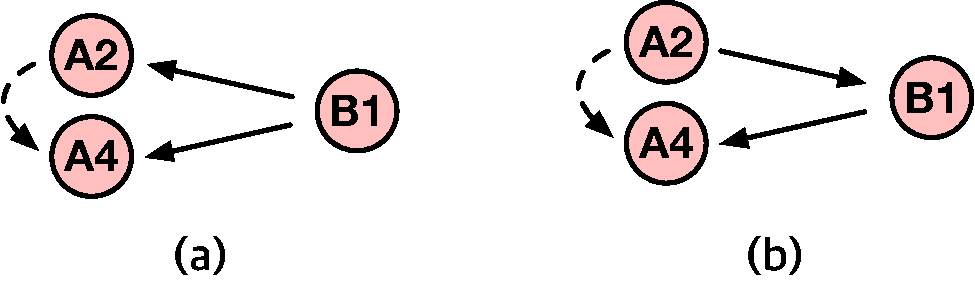
\includegraphics[width=0.7\linewidth]{fig/segmenthash.pdf}
  \caption{Two different interleaving segment graphs representing
    different interleavings of \texttt{A2}, \texttt{A4}, and
    \texttt{B1} from \autoref{fig:cve-2017-17712}.}
  \label{fig:segmenthash}
\end{figure}
%

In order to distinguish different interleavings of the same vertices,
we adopt Merkel hashing~\cite{treehashing, treehashing2}.
%
In particular, given a graph $G = (V, E)$, for all vertices $v \in V$,
we first calculate a hash value of $v$, $hash(v)$, which reflects its
out-going edges.
%
Let us denote $o_1, ..., o_m$ as vertices that is connected by an edge
$v \rightarrow o_x$. Then, $hash(v)$ is calculated as follow:
%
%
\\
\[
  hash(v) = \mathcal{H}(v.label {++} o_1.label {++} ... {++}
  o_m.label)
\]
\\
%
where $\mathcal{H}$ denotes the non-cryptographic FNV hash
function~\cite{fnv, fnv-go}, and ${++}$ denotes the
label-concatenation operation.
%
Then, $hash(G)$ is defined as follows:
%
\\[1pt]
\[
  hash(G) = \underset{v \in V}{\oplus} hash(v)
\]
\\[1pt]
%
where $\oplus$ denotes the XOR operation.

Applying $hash(G)$ to \autoref{fig:segmenthash}, $hash(\texttt{B1})$
is calculated as
$\mathcal{H}(\texttt{B1} ++ \texttt{A2} ++ \texttt{A4})$ in
\autoref{fig:segmenthash}-(a), whereas, $hash(\texttt{B1})$ is
calculated as $\mathcal{H}(\texttt{B1} ++ \texttt{A4})$ in
\autoref{fig:segmenthash}-(b).
%
Thus, hash values of even vertices labeled same (\ie, corresponding to
the same instruction) are calculated differently according to edges
connected to the vertex.
%
Likewise, values of $hash(\texttt{A2})$ are also calculated
differently in the two graphs as the direction of edges connecting
\texttt{A2} and \texttt{B1} is different in the two graphs.
%
As a consequence, values of $hash(G)$ (which are calculated as
$hash(\texttt{B1}) \oplus hash(\texttt{A2}) \oplus hash(\texttt{A4}$))
of \autoref{fig:segmenthash}-(a) and (b) are different, and \sys can
distinguish the two graphs in \autoref{fig:segmenthash} using hash
values of the two graphs.



\subsection{Input Transformation}
\label{s:appendix:inputtransform}



\subsection{Virtual Machine Introspection}
\label{s:appendix:vmi}

The execution engine introspects the target kernel for two reasons: 1)
the execution engine determines whether the breakpoint is hit by a
thread of the userspace fuzzer, or by an irrelevant thread, and 2)
when a running thread tries to acquire a lock, the execution engine
inspects whether the lock is held by a suspended thread.

As a hardware breakpoint does not distinguish the running context of a
kernel, if the context switch happens, a breakpoint may be hit by
another thread or an interrupt handler, making the execution out of
expectation.
%
The execution engine recognizes a running context using
\texttt{task_struct} which holds the thread description, and the
per-cpu \texttt{preempt_count} variable indicating what context the
thread is in (\eg, a task context for running a syscall, or a hardIRQ
context to handle hardware interrupts).
%
If a breakpoint is hit by a context other than the fuzzer-controlled
thread, the execution engine ignores it and keeps the breakpoint.


In addition, when the suspended thread already acquires a lock while
the running thread wants to hold the same lock, the whole execution
cannot make a progress, because the execution engine forces the
lock-holding thread to suspend.
%
Therefore, the execution engine inspects whether the running thread is
going to be blocked due to the lock contention, and if it is, the
execution engine takes control from the running thread to the
suspended thread.
%
Inspecting the lock contention is conducted by hooking lockdep
functions (\ie, \texttt{lock_acquire()} and \texttt{lock_release()} in
\texttt{kernel/locking/lockdep.c})~\cite{lockdep} that are commonly
called from synchronization primitives.
%
When the lockdep functions are called, the execution engine determines
whether the running thread can make a progress through various
information such as the address of the synchronization primitive, and
operation type (\ie, lock, unlock, and trylock).
%
If the running thread cannot make a progress, the execution engine
perform preemption to prevent unexpected block.

\subsection{Non-data race concurrency bug}
\label{s:appendix:datarace}

Data races are a subset of concurrency bugs as described in the
follow.


\begin{figure}
  \centering
  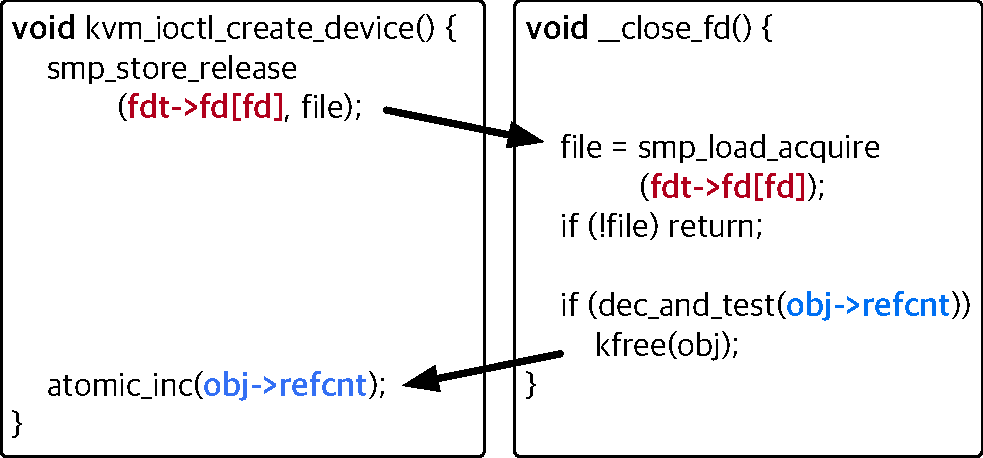
\includegraphics[width=0.85\linewidth]{fig/racecondition.pdf}
  \caption{Example of non-data race concurrency bug (CVE-2019-6974)
    found in the KVM submodule. Arrows denote the offending
    interleaving to cause a use-after-free bug.}
  \label{fig:concurrencybugs}
\end{figure}


\PP{Data race.}
%
Although the concept of data race is well known, its formal definition
depends on a programming language~\cite{C-standard-n2310,
  java-standard} or a program in development~\cite{lkmm}. In this
paper, we employ the definition from Linux Kernel Memory Model
(LKMM)~\cite{lkmm} released in 2018. According to LKMM, a data race
occurs when there are two memory accesses such that 1) they access the
same memory location, 2) at least one of them is a store, 3) at least
one of them is not annotated with special APIs such as
\texttt{WRITE_ONCE()}, or \texttt{smp_load_acquire()}, 4) they occur
on different CPUs (or in different threads on the same CPU), and 5)
they execute concurrently.
%
Informally, a data race indicates un-annotated concurrent accesses to
a shared memory location.

Data races are problematic because they may confuse a compiler.  LKMM
allows a compiler to assume that there will be no data race during the
runtime. Based on the assumption, a compiler has its rights to
arbitrarily transform plain accesses (\ie, accesses not annotated with
above operations), making the results unpredictable if there is a data
race during the runtime.
%
Therefore, LKMM defines the outcome of the program as undefined
behavior if a data race occurs.
%
Also, to prevent such undefined behaviors, LKMM requires developers to
annotate accesses if they possibly run
concurrently~\cite{data-race-fix1, data-race-fix2, data-race-fix3}.


% \PP{Race condition.}
% %
% Race condition is another type of concurrency bug. While a race
% condition broadly indicates that an outcome differs depending on the
% timing of concurrent events, we restrict the definition to indicate
% the correctness of the outcome differs according to the timing of
% concurrent events.
% %
% Specifically, if developers do not take consider of all possible
% interleavings, a program may execute an erroneous interleaving which
% leads the program into an unintended state.
% %
% Immediately or after a certain amount of time, the unintended state
% causes erroneous behaviors of the program such as memory corruption,
% deadlock, and assertion violation.

% \dr{TODO: what more?}
% In order to fix the errorneous interelaving, developers often utilize
% synchronization primitives such as a lock, or switch the order of
% instructions in a program~\cite{learningfrommistakes}.


% https://stackoverflow.com/questions/11276259/are-data-races-and-race-condition-actually-the-same-thing-in-context-of-conc
%
\PP{Example of non-data race concurrency bug}
%
\autoref{fig:concurrencybugs} shows the examples of non-data race
concurrency bug (\ie, CVE-2019-6974).
%
In \autoref{fig:concurrencybugs}, there is no data race because
reading from and writing to \texttt{fdt->fd[fd]} and
\texttt{obj->refcnt} is annotated with dedicated APIs such as
\texttt{smp_load_acquire()} and \texttt{dec_and_test()}.
%
In the perspective of data race detectors, all concurrent accesses are
out of the definition of data race, thus, data race detectors report
nothing with this example.
%
However, depending on interleaving of the two functions
\texttt{kvm_ioctl_create_device()} and \texttt{__close_fd()}, a
use-after-free bug may occur as described in the figure.



\PP{Scope of this paper}
%
\sys mostly focuses on finding concurrency bugs (including data races)
that exhibit harmful behaviors (\eg, memory corruptions). Thus, \sys
can easily detect \autoref{fig:concurrencybugs}, while data race
detectors cannot.
%
However, as Krace said, data race detectors are still valuable,
because there are data races that do not exhibit observable harmful
behaviors (\ie, performance degradation).
%
We believe integrating data race detectors into \sys reinforces the
\sys's bug-finding capability, and leave it as future work.


%%% Local Variables:
%%% mode: latex
%%% TeX-master: "p"
%%% End:
